\documentclass[10pt]{article}
\usepackage[margin=1in]{geometry}
\usepackage{booktabs}
\usepackage{graphicx}
\usepackage{amsmath,amssymb}
\usepackage{lmodern}
\usepackage[T1]{fontenc}
\usepackage{microtype}
\usepackage{xcolor}
\usepackage[hidelinks]{hyperref}
\usepackage{natbib}
\bibliographystyle{plainnat}

% Shared macros. Names and numbers that appear more than once live here so that a
% value cannot drift between two mentions of it.

\newcommand{\pns}{prior-normalised skill}
\newcommand{\pss}{patient-specific skill}
\newcommand{\Pns}{Prior-normalised skill}
\newcommand{\Pss}{Patient-specific skill}

% The two objects previously both called "fitted template". Never write either
% phrase inline; renaming one edits these four lines and nothing else.
\newcommand{\maskref}{mask-fitted reference}        % fit to validation lesion masks; the content-free ceiling
\newcommand{\Maskref}{Mask-fitted reference}
\newcommand{\attden}{attention-fitted denominator}  % reference_baselines.fitted_template; fit to the arm's own attention
\newcommand{\Attden}{Attention-fitted denominator}

% Numbers quoted more than once, from the confirmatory artefacts.
\newcommand{\maskrefInplane}{0.8302}   % masks:inplane flat AUC
\newcommand{\maskrefSep}{0.8543}       % masks:separable flat AUC
\newcommand{\attdenMedian}{0.4208}     % median attention:inplane over the 40 H5 dumps
\newcommand{\probeDen}{0.8358}         % the probe's attention-fitted denominator
\newcommand{\centrePriorSlice}{0.6427} % model-free centre prior, slice AUC, \condA{}
\newcommand{\armSlot}{slot arm}

\newcommand{\preghash}{\texttt{4fd6e801157ecef5}}
\newcommand{\repourl}{https://github.com/BhaveshThapar/SlotMIL}

\newcommand{\armNG}{Normal Guidance}
\newcommand{\armGA}{gated ABMIL}
\newcommand{\condA}{\texttt{nodule\_present}}
\newcommand{\condB}{\texttt{malignancy}}
\newcommand{\condC}{\texttt{balanced\_presence}}
\newcommand{\condD}{\texttt{mosmed\_severity}}

% A verdict, typeset so a FAIL is never quieter than a PASS.
\newcommand{\PASS}{\textsc{pass}}
\newcommand{\FAIL}{\textbf{\textsc{fail}}}
\newcommand{\RPT}{\textsc{reported}}


\title{Position priors dominate instance-level localisation metrics for\\
weakly-supervised multiple-instance learning in volumetric CT}
\author{Bhavesh Thapar\\University of Maryland\\\texttt{bthapar@terpmail.umd.edu}}
\date{}

\begin{document}
\maketitle

\begin{abstract}
Attention-based multiple-instance learning (MIL) is routinely credited with
localising findings in volumetric CT on the strength of instance-level AUC
against expert masks. We report a pre-registered evaluation of what that number
measures. Across ten MIL architectures on LIDC-IDRI, five seeds each, no arm's
flat (3D) instance AUC separates from its within-slice AUC by more than $0.02$,
no arm reaches a model-free centre prior on the axial axis, the $95$th percentile
over $30$ untrained initialisations is $0.7666$ --- so $0.5$ is not the floor ---
and a content-free in-plane template fit on validation reaches $0.8543$, above
every trained arm. Attention scored against a \emph{different} patient's masks
beats scoring it against the right ones for five of eight arms.
The single exception is the paper's second finding: an arm that injects an
explicit axial prior raises \pss{} by $+0.1509$ against a pre-registered
falsifier of $0.02$, and is independently the only arm the axis gate flags as
carrying axial content. Explicit prior injection, not architecture, is what adds
measurable localisation --- our instrument adjudicates that fix rather than
competing with it. We import two prior-normalised estimands from the saliency
literature and gate them on a supervised patch probe, which separates
($0.7305$) from every content-free baseline ($\leq 0.0105$) on the condition
carrying the hypothesis family; we recommend the estimands only where that
per-condition gate passes, and report that it fails on our $38$-bag condition
($0.4772$ against a $0.50$ bar). Finally, which axis carries the prior is a
property of the dataset, not of volumetric CT: our stereotypy hypothesis
predicted the ordering and was reversed by the data, with COVID ground-glass
\emph{more} positionally stereotyped than a lung nodule and stereotyped on the
axis LIDC leaves empty. We recommend a one-line convention any paper can adopt:
report raw and in-organ instance AUC side by side, and read the gap as that
dataset's positional confound.
\end{abstract}

% ==========================================================================
\section{Introduction}

Weakly-supervised MIL is trained on a bag-level label and is then asked, at
evaluation time, to say \emph{where} the finding is. The standard evidence is an
instance-level AUC: score every instance in a bag by its attention weight, label
instances by whether they intersect an expert mask, and pool. On volumetric CT
the instances are patch tokens over a stack of slices, and the resulting number
is reported as three-dimensional localisation.

This paper asks what that number is made of, and answers with three claims.

\paragraph{(i) The reported 3D localisation metric is largely in-plane
anatomical position.} Flat instance AUC over a whole volume is statistically
indistinguishable from within-slice AUC for seven of eight scored arms, so
nothing is being measured across the axial axis. A content-free reference that
reads no image at all --- a $256$-number in-plane template fit on validation ---
scores above every trained arm, and an untrained network reaches $0.7666$ at the
$95$th percentile. The apparent skill sits between a floor that is nowhere near
$0.5$ and a ceiling set by geometry.

\paragraph{(ii) The one intervention that adds real localisation is explicit
prior injection, and two tests that were not designed to agree both find it.}
Harvey-style \armNG{}~\citep{harvey2026b} adds a KL term pulling the attention's
slice marginal towards a moment-matched Normal. It is the only arm whose
\pss{} is raised past its falsifier, and independently the only arm the axis
gate flags as carrying axial content. Those are different statistics computed
from different artefacts; their agreement on one arm out of eight is a
replication, not a restatement. The critique fails for that arm, and we report
it as a failure --- but the more useful reading is that our instrument validates
their fix against a stronger reference than the one they used.

\paragraph{(iii) Which axis carries the prior is a property of the dataset.} We
pre-registered a prediction that prior dominance would track positional
stereotypy and that a lung nodule would be the more stereotyped finding. The
prediction was reversed with power to spare. COVID ground-glass is peripheral
and posterior in-plane and basal along the axis, and both show up: on MosMed the
mask-fitted axial template reaches slice AUC $0.8455$ against LIDC's $0.6180$.
``An in-plane metric wearing 3D clothing'' is a statement about LIDC. On another
cohort the confound lives somewhere else, which is precisely the argument for
measuring it per dataset rather than inheriting it.

\paragraph{Contributions.} Two prior-normalised estimands imported from the
saliency literature~\citep{kummerer2015,borji2013,bylinskii2019}; a validated
power gate showing they discriminate, with an explicit per-condition scope; a
pre-registered ten-hypothesis evaluation of ten MIL arms over four declared
conditions and two datasets; and a portable reporting convention that costs one
organ segmentation and no retraining.

% ==========================================================================
\section{Setup}

\paragraph{Data.} LIDC-IDRI~\citep{armato2011lidc}: $999$ series over $991$
patients, split $700/149/150$ by patient at seed $2027$ --- a split the analysis
protocol was never developed against. Frozen DINOv2 ViT-B/14
features~\citep{oquab2024dinov2}, $16\times16$ patch grid per slice, $768$
dimensions, giving bags of up to ${\sim}43.8$k instances. Instance labels come
from the four-radiologist consensus masks rasterised to the patch grid.
MosMed~\citep{morozov2020mosmed} enters for one hypothesis only: $50$ of $1110$
studies carry masks, all at severity CT-1, so re-splitting would leave too few
in test to estimate anything.

\paragraph{Conditions.} Four are declared. \condA{} carries the hypothesis
family and the multiplicity correction; \condB{} and \condC{} are LIDC
consistency checks; \condD{} runs the content-free template family only and
supports the stereotypy contrast. Which condition leads was ruled on
2026-08-15, before any confirmatory number existed, so that choosing after
seeing three verdict tables was not available.

\paragraph{Arms.} Ten: mean pooling, ABMIL~\citep{ilse2018}, gated ABMIL,
multi-head ABMIL, CLAM-SB~\citep{lu2021clam}, DSMIL~\citep{li2021dsmil},
TransMIL~\citep{shao2021transmil}, slot attention~\citep{locatello2020slot} with
a diversity term, and the two Harvey arms --- a fixed centre
Gaussian~\citep{harvey2026a} and \armNG{}~\citep{harvey2026b}. Five seeds each.
Mean pooling and the centre Gaussian have attention fixed by construction and
are reported but not scored, so the scored set is eight.

\paragraph{Statistics.} Every AUC is a patient-clustered bootstrap over per-bag
AUCs, $10{,}000$ replicates. Where a hypothesis states a per-arm bound without a
unit over seeds, we take the mean over seeds and record that we took it
(\S\ref{sec:limits}).

% ==========================================================================
\section{Estimands}

Two estimands are imported rather than invented.

\paragraph{\Pns{}} $\;s = (A - A_t)/(1 - A_t)$, the fraction of the headroom
above a content-free reference that a method claims; structurally the
information-gain-over-a-baseline construction
of~\citet{kummerer2015}, kept on the AUC scale so it reads against published
tables. The reference $A_t$ is pre-registered as an in-plane template fit on
validation --- tighter than an unfit average mask~\citep{arun2021saliency} and
tighter than a fixed $\sigma{=}1$ Gaussian~\citep{harvey2026a}, so it shrinks the
denominator and lowers every reported skill, which is the honest direction.

One property of that reference is worth stating in advance, because it is the
mechanism and not a defect. The template is fit to \emph{the arm's own
attention}. Fit to the supervised probe's output the identical rule scores
$0.836$; fit to a MIL arm's attention its median over the scored dumps is
$0.4208$, below chance, because their attention carries no in-plane structure to
fit. A sub-chance denominator inflates $1 - A_t$ above $1$ and so shrinks the
reported skill, which makes a hypothesis that passes by staying \emph{below} a
bar easier to pass. We report the conservative recomputation in
\S\ref{sec:h4h5}.

\paragraph{\Pss{}} $\;A_{\text{real}} - A_{\text{cross-patient}}$, the
score that survives swapping whose masks the attention is scored
against~\citep{borji2013,bylinskii2019}; the model, protocol and selection step
are held identical and only the target changes.

% ==========================================================================
\section{Results}

\begin{figure}[t]
\centering
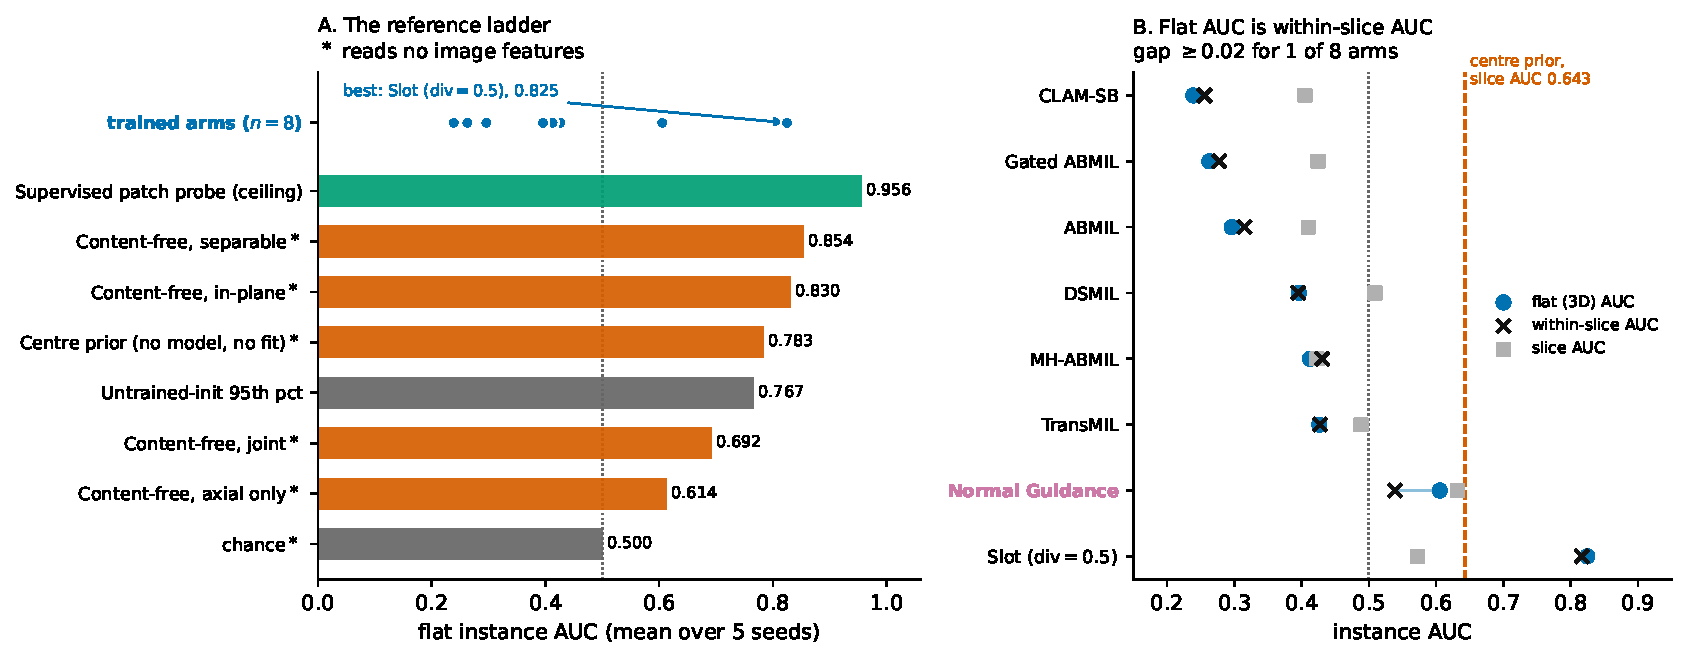
\includegraphics[width=\textwidth]{figures/fig1_reference_ladder.pdf}
\caption{\textbf{Left:} the reference ladder on \condA{}. Starred references read
no image features at all --- they are computed from lesion masks and patch
geometry. The best trained arm sits below the content-free separable template
and barely above an untrained network's $95$th percentile.
\textbf{Right:} flat, within-slice and slice instance AUC per scored arm. Flat
and within-slice coincide for every arm but \armNG{}, and no arm's slice AUC
reaches the model-free centre prior.}
\label{fig:ladder}
\end{figure}

\subsection{The floor, the ceiling, and the axis (H1--H3)}

\paragraph{H1 (lead), \PASS{}.} $|{\text{flat}} - {\text{within-slice}}|$ exceeds
$0.02$ for $1$ of $8$ arms; the falsifier required a majority, $5$. The harness
validates itself first: the positive controls do separate --- \texttt{masks:axial}
$0.1064$, \texttt{centre\_prior} $0.0518$, \texttt{masks:separable} $0.0234$ ---
and the tie floor for uniform attention is exactly $0.0$, so the test can detect
axial content when it is present. The one arm over the bar is \armNG{} at
$0.0669$, next-highest ABMIL at $0.0190$: a $3.5\times$ separation.
The reported 3D localisation metric is an in-plane metric wearing 3D clothing.

\paragraph{H2, \PASS{}.} No trained arm reaches the model-free centre prior's
slice AUC of $0.6427$; the best is \armNG{} at $0.6318$. A prior with no
parameters and no fitting beats every trained arm on the axis.

\paragraph{H3, \PASS{}.} The $95$th percentile instance AUC over $30$ untrained
initialisations is $0.7666$, against a bar of $0.70$, taken as the weaker of two
poolings. Chance is not the floor for this protocol, and a reported $0.79$--$0.82$
is inside the untrained range.

\subsection{What survives normalisation (H4, H5)}
\label{sec:h4h5}

\paragraph{H4, \PASS{}, and more strongly than claimed.} Median \pss{} is
$-0.0466$ and five of eight arms are negative --- scoring an arm's attention
against another patient's masks \emph{beats} scoring it against the right ones.
The falsifier only required every arm below $0.15$ and the median below $0.10$.

\paragraph{H5, \PASS{}.} No arm's \pns{}, as the mean over seeds, exceeds
$0.30$; the maximum is the slot arm at $+0.1990$. One individual seed sits above
the bar at $0.3432$ and is reported rather than absorbed, because the unit was
declared before that seed existed.

\paragraph{H5 under a floored denominator (not pre-registered).} Because the
declared denominator sits below chance for $24$ of $40$ scored dumps
(\S3), we recompute the identical statistic --- floor per tag, mean over seeds,
maximum over the arm set --- with the denominator floored at $0.5$, outside the
confirmatory family and without amending the frozen configuration.

\begin{center}
\begin{tabular}{lccc}
\toprule
Condition & max skill, as published & denominator floored at 0.5 & bar \\
\midrule
nodule\_present & +0.1990 & +0.1990 & 0.3 \\
malignancy & +0.2812 & +0.2304 & 0.3 \\
balanced\_presence & +0.0885 & +0.0220 & 0.3 \\
\bottomrule
\end{tabular}

\end{center}

\noindent The verdict does not move in any condition, and flooring \emph{lowers}
the maximum wherever it binds. The caveat cuts against us and the conservative
recomputation removes it.

\subsection{The power gate, and its scope (H7)}

A critique whose estimands score zero for everything is not a fix, so the
constructive half of the paper is gated on a pre-registered test: a supervised
patch probe must clear $0.50$ \pns{} while every content-free baseline stays
below $0.05$.

\paragraph{H7, \PASS{} on \condA{}.} The probe reaches $0.7305$
($A = 0.9558$ against its own template at $0.8358$). The content-free set:
chance $0.0$, roll permutation $+0.0105$, entropy-matched random $-0.0001$,
fitted template $0.0$ by construction. The estimands discriminate.

\paragraph{Scope, stated up front.} The gate is per condition, and it does not
pass everywhere: \condA{} $0.7305$, \condB{} $0.7036$, \condC{}
$\mathbf{0.4772}$ against the $0.50$ bar. On \condC{} the probe's own in-plane
template is the strongest of the three ($0.8568$) while its AUC is the weakest
($0.9252$), so the headroom the ratio measures is genuinely small --- a statement
about $38$ test bags, not about the estimand. \textbf{We recommend the
estimands only where the per-condition gate passes.} Where it fails, report the
raw and in-organ AUCs of \S\ref{sec:h8} instead.

\paragraph{How H7 was measured, and what was known when.} The two stochastic
content-free members were originally computed \emph{once} per tag: the generator
was rebuilt per tag with a fixed seed, so every tag in a condition shared one
realisation and no draw-to-draw variance was estimable anywhere. Under that
construction the gate --- a maximum over tags --- returned $0.0784$ and H7
\textbf{failed}. We do not claim the pass holds on the single-draw form; it does
not, on the original arm set or the current one. The amendment of 2026-08-17
replicated each member $30$ times per tag and took the mean over draws, and four
properties of how it was written are what make the result usable. It was drafted
and committed \emph{before} the replicated numbers existed, and says so; the full
pre-amendment table under mean, median and max was known, and showed the gate
clearing under mean or median in every condition and failing under max in every
condition. It left the \emph{stricter} aggregation --- the maximum --- in force.
Draw $0$ is seeded exactly as the single-draw form was, so the published
realisation stays locatable inside its own distribution. And decisively, the
replicated per-tag draw-to-draw standard deviation reaches $0.0673$ on the
condition carrying the family, against the $0.05$ threshold the single draw was
being compared to: a maximum over one draw from a distribution whose spread
exceeds the threshold is not an unlucky measurement, it is not a measurement.
The verdict artefact carries the mean/median/max sensitivity table so the choice
is checkable rather than assertable.

\subsection{Prior injection is the exception (H6)}

\begin{figure}[t]
\centering
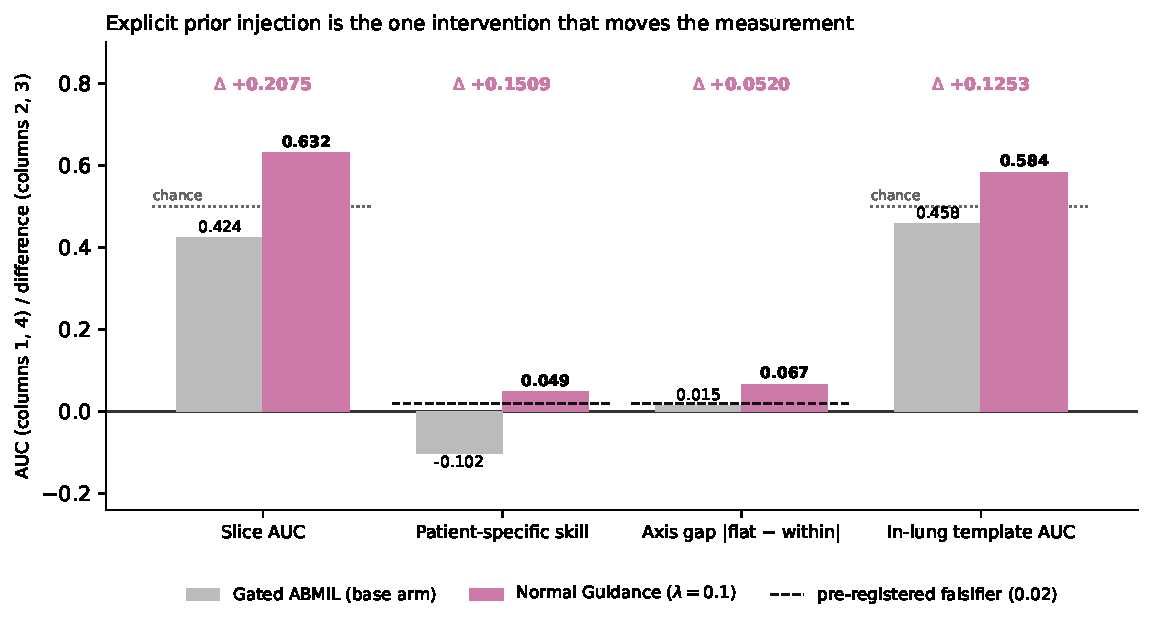
\includegraphics[width=0.86\textwidth]{figures/fig2_normal_guidance.pdf}
\caption{\armNG{} against its own base arm, \armGA{}, on four axes. The KL term
is the only difference between the two. Columns 1 and 4 are AUCs; columns 2 and 3
are differences.}
\label{fig:ng}
\end{figure}

\paragraph{H6, \FAIL{}, and the failure is the paper's second finding.} The
falsifier stated that if \pss{} rises by $\geq 0.02$ then prior injection is
adding real information and the critique fails for that arm. It rose by
$+0.1509$, from $-0.1019$ to $+0.0490$. We report that as a failure.

Three things make it more than a caveat. First the magnitude: \armNG{} is one of
only three arms with positive \pss{} at all (with the slot arm at $+0.0740$ and
TransMIL at $+0.0177$), and the only one that also clears the axis gate. Second
the independence: H1's axis gate reads \texttt{axis\_gate.json} and H6's skill
reads \texttt{h4\_cross\_patient.json}; they are different statistics on
different artefacts and both single out the same arm out of eight. It also holds
on \condC{}, where \armNG{} is again the only arm over the bar. Third the
mechanism: the arm's only departure from \armGA{} is a KL term pulling the
attention's slice marginal towards a moment-matched Normal over slice index, so
a gain cannot be attributed to a stronger backbone or to rescuing a weak base.
Nothing in the architecture sweep adds localisation; a loss term that names the
axial coordinate explicitly does.

\paragraph{And what it does not show.} \armNG{}'s slice AUC of $0.6318$ still
does not reach the model-free centre prior at $0.6427$, so H2 holds for it too.
Prior injection is the only thing in this sweep that moves the measurement; it
does not solve the problem.

\subsection{The portable convention (H8)}
\label{sec:h8}

\begin{figure}[t]
\centering
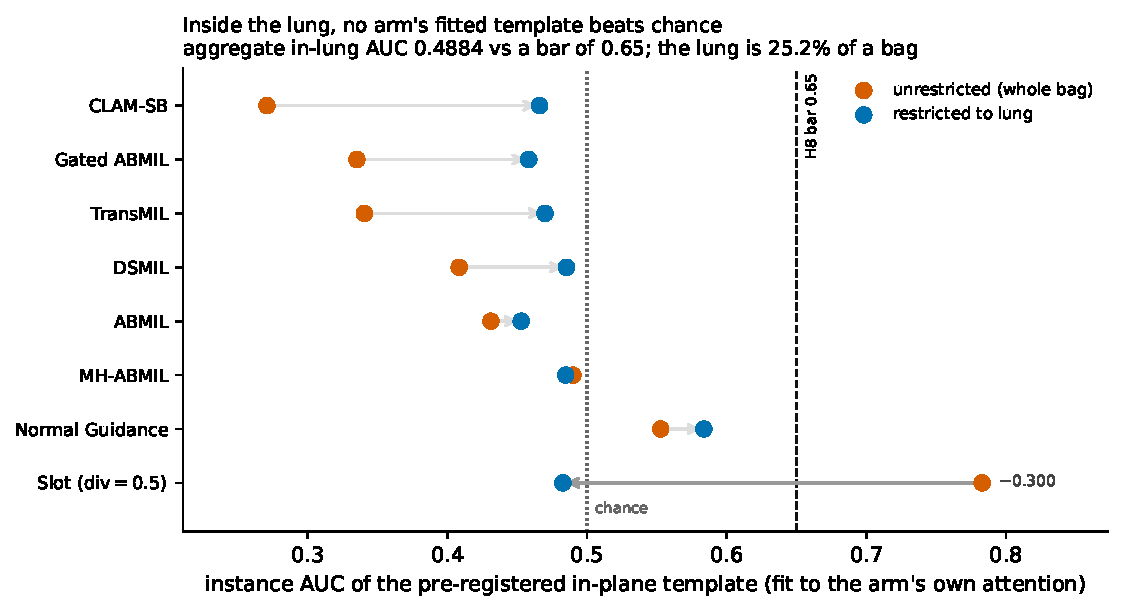
\includegraphics[width=0.86\textwidth]{figures/fig4_in_lung.pdf}
\caption{The pre-registered in-plane template, scored on the whole bag and
restricted to a lung segmentation. Note the scored quantity is the template fit
to each arm's attention, not the arm's own attention: for most arms it is already
at chance unrestricted, so only the arms whose template carried in-plane
structure have anything to lose.}
\label{fig:lung}
\end{figure}

H8 was declared two-sided with no falsifier, and with it written in advance that
if restricting to lung removed the prior, that would become the paper's
recommendation rather than a defeat. It does. The lung is $25.2\%$ of a bag, and
inside it the pre-registered template scores $0.4884$ against a bar of $0.65$,
with the position-stratified variant at $0.4936$ beside it and all three
conditions agreeing ($0.4884 / 0.5080 / 0.4940$). No arm's fitted template beats
chance inside the lung.

\paragraph{Recommended convention.} \textbf{Report raw and in-organ instance AUC
side by side, and read the gap as that dataset's positional confound.} It costs
one organ segmentation and no retraining, it is interpretable without any
estimand this paper proposes, and it is the one recommendation here that applies
where the power gate fails.

\subsection{The dataset contrast, and a prediction we got wrong (H9)}

\begin{figure}[t]
\centering
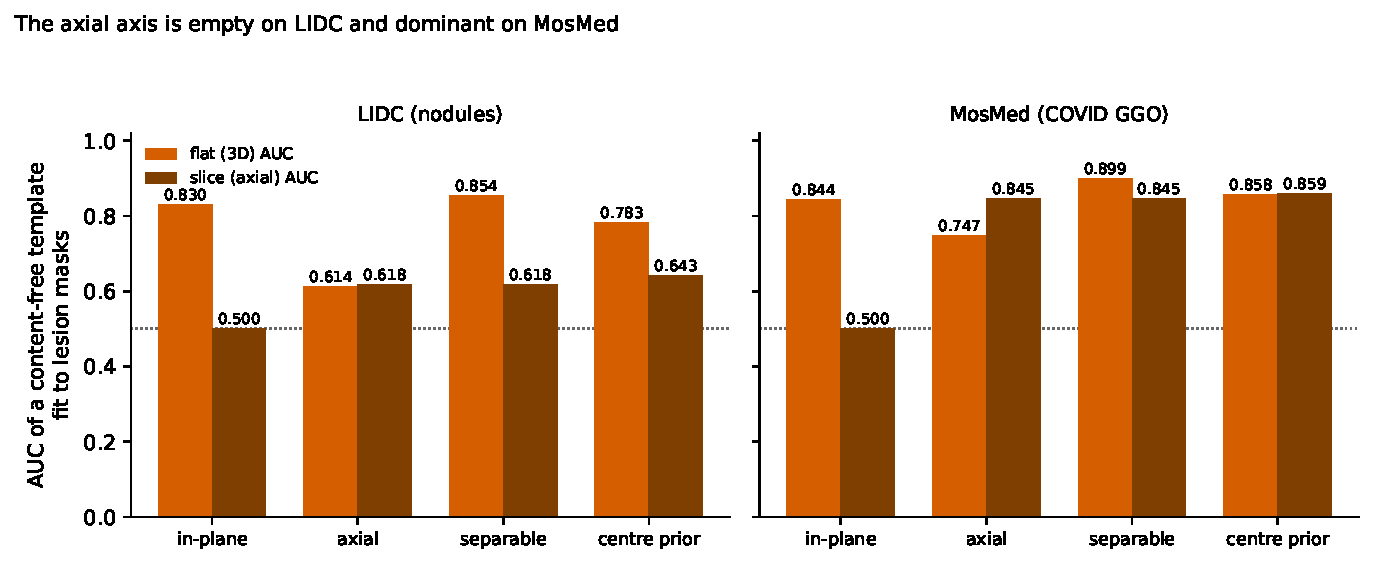
\includegraphics[width=\textwidth]{figures/fig3_dataset_contrast.pdf}
\caption{Content-free templates fit to lesion masks, LIDC versus MosMed. The
axial axis is empty on LIDC and dominant on MosMed. No training is involved in
any bar.}
\label{fig:contrast}
\end{figure}

\paragraph{H9, \FAIL{}, and reversed.} H9 predicted that prior dominance would
track positional stereotypy, treating a lung nodule as the more stereotyped
finding, and required MosMed's fitted-template AUC to sit below LIDC's with the
intervals separated. One of $50$ matched (arm, seed) pairs clears that; two order
on the point estimate alone. The two counts are the artefact's \texttt{reason}
and \texttt{power.n\_ordering} respectively and they measure different things.
The failure is not a lack of power: the median observed separation is $-0.2495$
against a median \emph{required} separation of $+0.0560$, over $22$ MosMed and
$129$ LIDC clusters. The sign is wrong, and tighter intervals would not rescue
it.

The mechanism we proposed was wrong in an instructive direction. LIDC nodules are
distributed through the parenchyma with little axial preference --- the
mask-fitted axial template reaches only $0.6136$ flat and $0.6180$ slice AUC,
against $0.8302$ for the in-plane member. COVID ground-glass is the opposite:
peripheral and posterior in-plane, basal along the axis, and both show up, with
MosMed's mask-fitted axial template at $0.7473$ flat and $0.8455$ slice and its
separable member at $0.8988$. The model-free centre prior tells the same story,
slice AUC $0.6427$ on LIDC and $0.8586$ on MosMed. COVID ground-glass is
\emph{more} positionally stereotyped than a lung nodule, and stereotyped on the
axis LIDC leaves empty. What was wrong was our operationalisation of stereotypy
as a property of a finding's size and dispersion rather than of its
organ-relative distribution; whether a better operationalisation would recover
the ordering is open, and we do not claim one here.

This is the strongest available argument for the protocol. We predicted prior
dominance from intuition about the findings, we were wrong with power to spare,
and only a per-dataset measurement caught it. An evaluation of MosMed that had
inherited LIDC's conclusion and controlled only the in-plane prior would have
left most of the confound in place. Which axis carries the prior must be measured
on the cohort being reported, and Figure~\ref{fig:contrast} costs no training to
produce for a new one.

\subsection{Multiplicity}

The declared Holm family~\citep{holm1979} is eight arms $\times$ three
references, $24$ comparisons per seed, corrected per seed; $15/15/15/16/14$ are
rejected. This must not be read as discrimination: at ${\sim}7.4$M pooled paired
instances the DeLong~\citep{delong1988} $p$ underflows to exactly zero for
$15/14/10/16/13$ of them, so every pairable member is rejected whatever the
multiplier. The cross-patient reference is a label-side null and has no paired
$z$ at all; it stays in the family at $p = \mathrm{NaN}$, preserving the family
size, and is never rejected.

% ==========================================================================
\section{Limitations}
\label{sec:limits}

\paragraph{One backbone.} Every result uses frozen DINOv2 ViT-B/14, and a second
backbone would strengthen the sweep. It would not change the central
measurement. The references that set the ceiling --- the mask-fitted in-plane
template at $0.8302$, the separable template at $0.8543$, the centre prior at
$0.7833$ --- \emph{read no image features at all}; they are computed from lesion
masks and patch geometry and are invariant to the encoder by construction. That a
content-free positional reference reaches the level of trained attention-MIL
localisation on LIDC therefore cannot be an artefact of feature choice. What a
second backbone could change is where the \emph{trained} arms land relative to
that fixed ceiling, and we do not measure it here.

\paragraph{Undeclared units.} Three hypotheses state a bound without a unit of
aggregation. H1 and H4 give a per-arm bound with no unit over seeds and are taken
as the mean over seeds --- H5's own rationale makes that argument for the
identical hole, and a per-seed maximum would take five draws at the threshold
instead of one. H9 states an ordering with no aggregation over arms and seeds and
is taken as every matched tag, the strictest available reading. All three are
recorded in the verdict artefact under \texttt{undeclared\_units\_taken} rather
than left implicit, and were chosen before the numbers they aggregate were read.

\paragraph{Power in the secondary conditions.} \condC{} has $38$ test bags over
$38$ patients, wide enough that most interval outcomes land
\emph{indistinguishable} by design; \condB{} has a supervised patch-probe ceiling
of $0.6516$ against \condA{}'s $0.9102$, so it tests the label rather than the
method. Both limits were stated at declaration, not discovered at analysis.
MosMed contributes $22$ annotated test scans.

\paragraph{Provenance.} The confirmatory sweep spans two commits, $95$ seeds and
$105$ seeds, all clean and all at one configuration hash; the diff between them
touches only the scoring script and its tests, no training-path file, so training
is bit-identical across the two. Disclosed rather than re-run.

% ==========================================================================
\section{Recommendations}

\begin{enumerate}\itemsep2pt
\item \textbf{Report raw and in-organ instance AUC side by side.} The gap is that
dataset's positional confound. One segmentation, no retraining, no new estimand.
\item \textbf{Report the axis decomposition.} Flat, within-slice and slice AUC for
the same scores. If flat equals within-slice, the metric is not measuring the
third dimension, and the reader can see it in one line.
\item \textbf{Measure the floor, do not assume it.} Report a content-free
positional reference and an untrained-initialisation percentile for the protocol
in use. Chance is not the floor.
\item \textbf{Normalise against a fitted reference, and gate it.} Report \pns{}
against an in-plane template fit on validation, and report the per-condition
supervised-probe gate beside it. Where the gate fails, fall back to
recommendation~1.
\end{enumerate}

% ==========================================================================
\section{Pre-registration}

Every threshold, arm and estimand in this paper was frozen in a machine-readable
pre-registration (configuration hash \preghash{}) before any confirmatory number
existed; the analysis code reads its parameters only from that file and raises on
anything undeclared, every result carries the configuration hash and git commit
it was produced under, and the complete falsifier table, the dated amendment
chain and the diff between what was declared and what was reported are in the
companion and at \url{\repourl}.

\begin{center}
\begin{tabular}{lcccccccccc}
\toprule
Condition & H1 & H2 & H3 & H4 & H5 & H6 & H7 & H8 & H9 & H10 \\
\midrule
nodule\_present$^\dagger$ & PASS & PASS & PASS & PASS & PASS & \textbf{FAIL} & PASS & RPT & \textbf{FAIL} & PASS \\
malignancy & PASS & PASS & PASS & PASS & PASS & \textbf{FAIL} & PASS & RPT & \textbf{FAIL} & PASS \\
balanced\_presence & PASS & PASS & PASS & PASS & PASS & \textbf{FAIL} & \textbf{FAIL} & RPT & \textbf{FAIL} & \textbf{FAIL} \\
\bottomrule
\end{tabular}

\end{center}
\noindent {\small $^\dagger$ carries the hypothesis family; the other two LIDC
conditions are consistency checks. RPT $=$ reported, two-sided by declaration.}

\bibliography{refs}
\end{document}
